\section{Museum Lighting}

\bigskip

\begin{quote}
`Museums and art galleries collect, preserve, and display natural artifacts and/or examples of human achievement and analyze their impact on the world and the universe around us. Effective exhibit lighting must balance exhibition and conservation needs and enrich the museum experience.'
\end{quote}

\begin{flushright}IES RP-30-96 Museum and Art Gallery Lighting: \\A Recommended Practice \citep{ies_ies_1996}\end{flushright}

\bigskip

Lighting in museums is required to satisfy multiple criteria; perhaps the least contestable requirement being that the lighting illuminate objects such that they are suitably visible to museum visitors. Also of utmost importance in most museum settings is that the lighting does not have an unreasonably damaging effect upon the objects or environment, be this through direct photodegradation or as a result of heat transfer. Further to these requirements, an increased or optimal visual quality is generally desirable, although what this represents or how to achieve it is generally ambiguous.

In sweeping terms, all electromagnetic radiation (visible and non-visible) damages objects, and more radiation damages objects proportionally moreso. Thus the question becomes: \emph{how little light can we use to illuminate objects such that they're visible to the extent required?} The inverse form, sometimes used on the assumption that more light always represents an increase in observer satisfaction/pleasure is: \emph{`how much light can we use so that only $x$ damage occurs over $y$ time'}. 

Industry guidance documents provide advice on how to manage lighting to best address the above requirements and many other additional specific requirements through the recommendation of procedure and provision of target figures for quantitative variables. \Gls{UV} radiation, being of no visual benefit but having potential to harm, is now excluded from gallery spaces as an industry standard.

\subsection{Damage functions} \label{sec:DamageIndex}

\textit{The key reference on this subject is CIE 157:2004 \citep{cie_cie_2004}, and valuable talks on the subject were given at the recent Museum Lighting Symposium \& Workshops\citep{pokorska_book_2017} (which the author helped to organise), and have been made freely available online\footnote{See in particular the talks by David Saunders (\url{https://www.youtube.com/watch?v=H4d0qH0IBcI&t}) and Stefan Michalski (\url{https://www.youtube.com/watch?v=XUY9biLQqlw})}.}.

\bigskip

In heritage science `damage functions' are ``functions of unacceptable change, dependent on agents of change''\citep{strlic_damage_2013}. The goal of damage functions in heritage lighting engineering is to give a quantitative means by which to predict the amount of damage caused to a prototypical object by a given light source, and to assist in limiting such damage. They generally follow the logic that radiation of lower wavelength is likely to cause more damage to objects.

\citet{harrison_report_1953} is generally acknowledged as the first to suggest such a function, but he himself acknowledges that it had ``long been established that the shorter the wavelength (visible yellow, green, blue, violet and invisible UV being progressively shorter) the more photochemically potent will be such radiant energy, provided such energy is actually absorbed''. \citet[p.9]{harrison_report_1953} defined the `radiation hazard associated with a light source' as:

\begin{equation}
    \sum_{0}^{\infty} \mathrm{H}_{\lambda} \mathrm{D}_{\lambda} \Delta \lambda / \sum_{0}^{\infty} \mathrm{H}_{\lambda} \overline{\mathrm{y}}_{\lambda} \Delta \lambda
    \label{eq:Harrison}
\end{equation}

where $\mathrm{H}_{\lambda}$ is the spectral irradiance, $\mathrm{D}_{\lambda}$ is the `Relative Damage Factor' (which is extrapolated from the data collected shortly prior to Harrison's own report by the National Bureau of Standards \citep{national_bureau_of_standards_preservation_1951}, and shown in Figure \ref{fig:Harrison}), and $\overline{\mathrm{y}}_{\lambda}$ is the CIE 1924 photopic $V_{\lambda}$ luminosity function. The resulting value would describe the amount of damage expected from a light source, normalised by its luminance.

\begin{figure}[htbp]
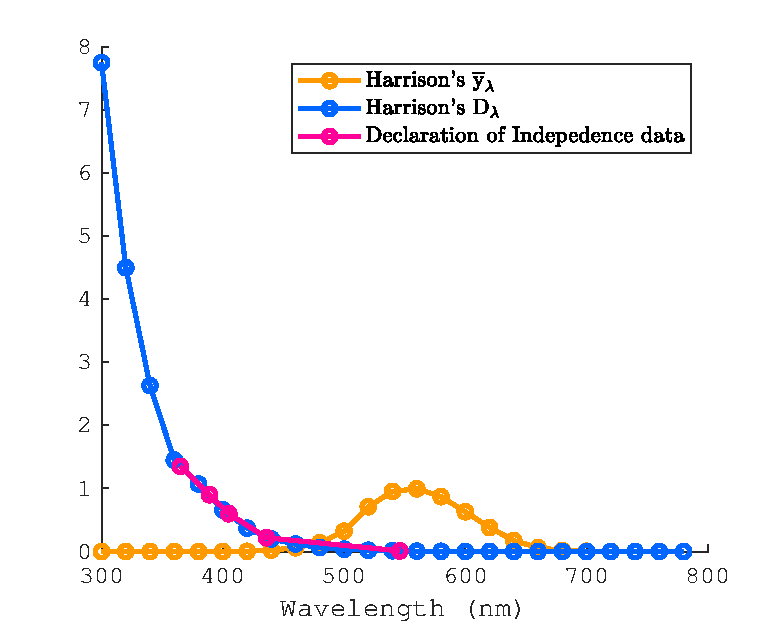
\includegraphics[max width=\textwidth]{figs/LitRev/HarrisonInd.pdf}
\caption{Harrison's \citep{harrison_report_1953} damage function ($\mathrm{D}_{\lambda}$), and luminous efficacy ($\overline{\mathrm{y}}_{\lambda}$), alongside the Declaration of Independence data \citep{national_bureau_of_standards_preservation_1951} from which it was extrapolated (re-normalised to match scale).}
\label{fig:Harrison}
\end{figure}

\begin{figure}[htbp]
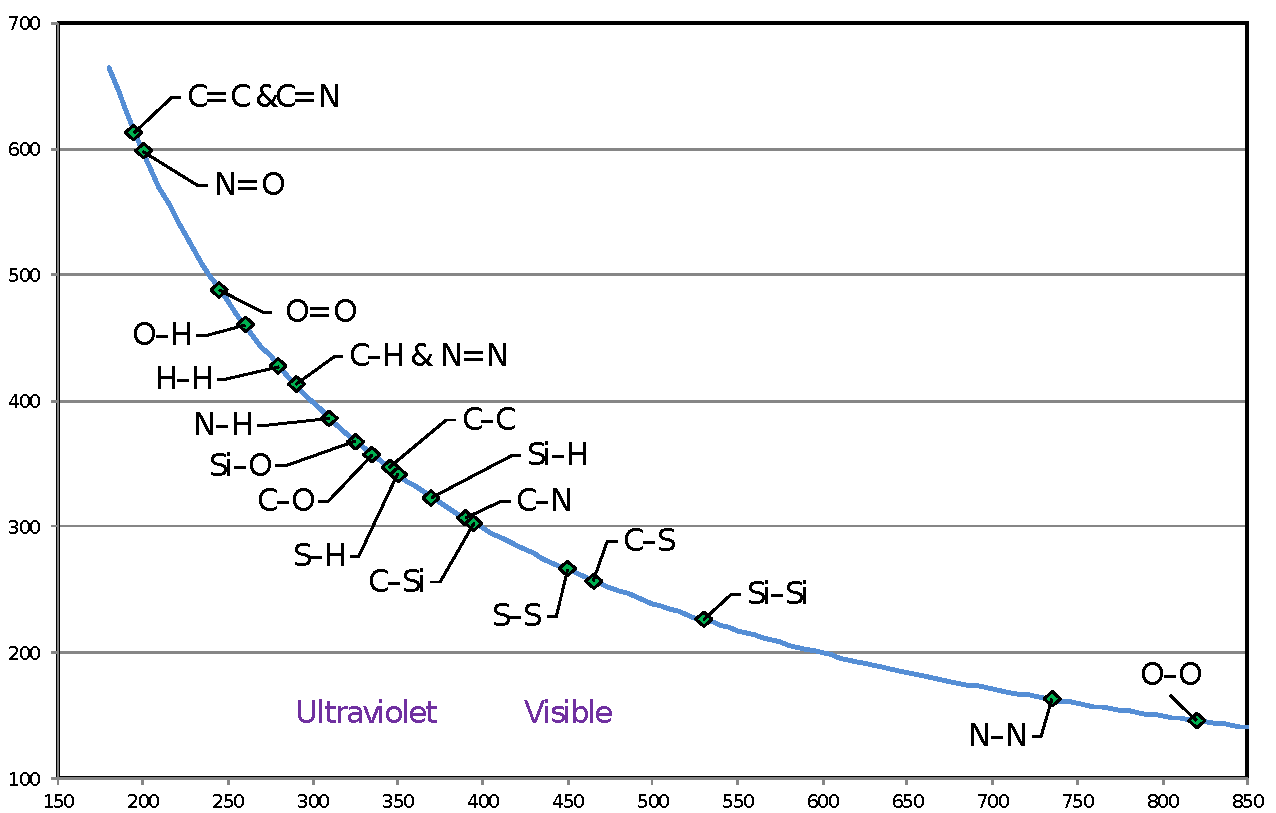
\includegraphics[max width=\textwidth]{figs/LitRev/Saunders.pdf}
\caption{Graph courtesy of David Saunders, presented at the Museum Lighting Symposium \& Workshops \citep[p.61]{pokorska_book_2017} showing the relationship between wavelength and the bonds which can be broken in various molecules, with `Wavelength (nm)' on the abscissa and `Bond energy (kJ/mol)' on the ordinate.}
\label{fig:Saunders}
\end{figure}

There has been extended scepticism about the utility of damage functions in general, with the argument being that no one damage function could represent the vast range and complexities of real materials. \citet[p. 178]{thomson_museum_1978} wrote that ``for more fugitive materials \dots the figure for visible radiation would be higher. On the other hand \dots the fastest dyes are probably affected only by UV. Thus it can be seen that no single figure can be given for damage versus wavelength''.

Criticism was aimed at this specific damage function due to it's derivation from such a small and minimally representative dataset - Harrison's data was `extended' from the 5 datapoints measured by the National Bureau of Standards \citep{national_bureau_of_standards_preservation_1951} in their investigations of how to best care for the Declaration of Independence\footnote{It is a curiosity that these minimal figures would not in fact have been much use to those planning the care for the declaration, since in the report it is noted that ``The deterioration of animal parchment is not as rapid as that of the low-grade paper for which the damage factors were determined''\citep{national_bureau_of_standards_preservation_1951}, and the Declaration of Independence is written on animal parchment.}, and was derived from the study of `low-grade paper', which cannot to said to represent the average museum item\footnote{Though \emph{no} material truly can!}.

CIE 157:2004 \citep{cie_cie_2004} notes that whilst Harrison's proposal failed to gain acceptance as the procedure for comparing the damage potential of different types of light sources, it did convince people of the ills of \gls{UV}, with the result that daylight was subsequently eliminated from many galleries.

Following \citet{cuttle_lighting_1988}, who noted that Harrison's damage function could be well fit by an inverted logarithmic function, with parameters controlling the slope and normalisation point of the function, CIE 157:2004 provided the following equation:

\begin{equation}
    s(\lambda)_{\mathrm{dm,rel}}=\exp [-b(\lambda-n)]
    \label{eq:damfac}
\end{equation}

where differing values of $b$ for 5 categories of item are provided (Table \ref{tab:b}), $n$ is the normalisation value (CIE 157:2004 uses a value of 300), and the $s(\lambda)_{\mathrm{dm,rel}}$ function is the estimated action spectrum for each category. $s(\lambda)_{\mathrm{dm,rel}}$ would be substituted into Equation \ref{eq:Harrison} for $\mathrm{D}_{\lambda}$. CIE 157:2004 also provides values of $H_{s,dm}$ which indicate the susceptibility of each group of materials to damage (where damage is considered as colour change%in $\Delta E_{\mathrm{ab}}^{\ast}$
).

\begin{table}[htbp]
\centering
\begin{tabular}{|c|l|l|l|}
\hline
Group & Samples & $H_{s,dm}$ (W h/m$^{2}$) & $b$ \\ \hline
a & Low-grade paper & 5 & 0.038 \\ \hline
b & Rag paper & 1200 & 0.0125 \\ \hline
c & Oil paints on canvas & 850 & 0.0115 \\ \hline
d & Textiles & 290 & 0.0100 \\ \hline
e & Water colours on rag paper & 175 & 0.0115 \\ \hline
\end{tabular}
\caption{Table reproduced from CIE 157:2004 \citep{cie_cie_2004}, showing the values for $H_{s,dm}$ and $b$ for various categories. Note: the source for this data is not particularly clear; it is listed as `The Berlin researchers', which is assumed to follow the references: \citet{krochmann_beleuchtung_1988,cie_cie_1991,hilbert_zur_1991}; none of which I have been able to access.}
\label{tab:b}
\end{table}

The more general criticism that damage functions will never be able to represent all museum objects is a valid concern, and can be well illustrated with the following logic: museums own objects of many different colours, different colours arise from different reflectance properties, different refelctance properties mean different wavelengths are absobed, and damage can only occur when radiation is absorbed. Thus it follows that one would expect two objects of different colours to have different damage functions. 

The classic study on how reflectance properties relate to damage is that of \citet{saunders_wavelength-dependent_1994}. They exposed a number of pigments to a range of wavelengths and measured the resulting damage. \citet{cuttle_control_1999} later replotted the data from this study (reproduced in Figure \ref{fig:Cuttle}), highlighting the apparent joint contributions of spectral reflectance and a general damage function to the individual damage functions. CIE 157:2004 notes however that this correspondence is not perfect or easily modellable, and that ``a workable system for characterising action spectra for colorants, including pigments and dyes, remains an unattained goal''. Recent studied have added new data (see esp. \citet{villmann_wavelength_2018}), and it is hoped that a general understanding may at some point be reached.

\begin{figure}[htbp]
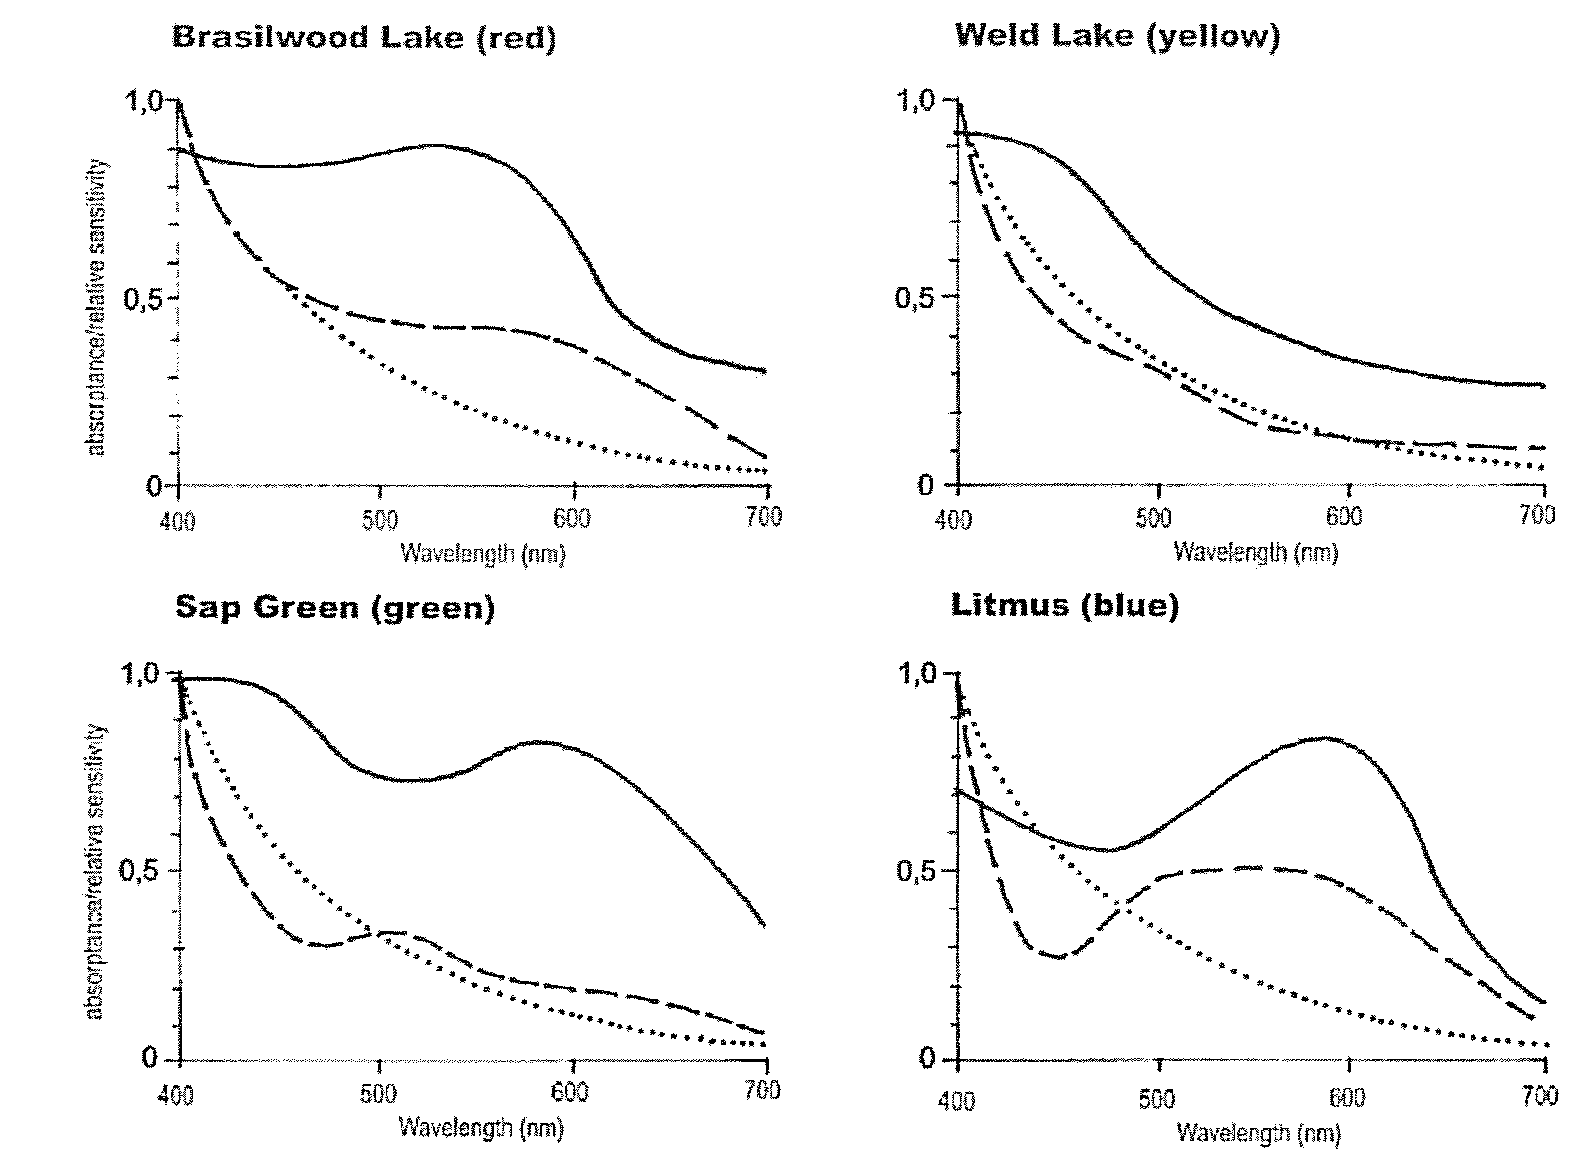
\includegraphics[max width=\textwidth]{figs/LitRev/Cuttle.png}
\caption{Figure of \citet{cuttle_control_1999}, using data from \citet{saunders_wavelength-dependent_1994}, and reproduced here from CIE 157:2004 \citep{cie_cie_2004}. Caption from CIE 157:2004 ``Spectral absorptance (solid line) and relative spectral responsivity (broken line) for artist's pigments \dots The dotted lines show relative spectral sensitivities normalised at 400nm based on the Berlin relative spectral responsivity function.''}
\label{fig:Cuttle}
\end{figure}

However, it is the opinion of this author that this argument is an exercise in artificial futility; whilst we may not be able to model the individual damage functions for every object in a museum, we may at least use one which has some bearing on the damage function, rather than the one which is implicitly used by museums currently - the CIE 1924 luminosity function ($\overline{\mathrm{y}}_{\lambda}$ of Figure \ref{fig:Harrison}), which relates to the sensitivity of the human eye rather than any type of object. \citet{cuttle_lighting_1988} puts it well: ``The argument, then, is not whether we have a [damage] function which is correct, but whether we can improve usefully upon the likely reliability of the present system''. It is depressing that this was said in 1988 and yet little seems to have changed in practice (See Chapter \ref{chap:Interviews}).

In the case where specific objects/pigments of interest can be identified, and their individual damage functions calculated, there is valuable recent research to draw on regarding methods for optimising light sources to minimise damage \citep{durmus_optimising_2017,durmus_colour_2015,durmus_optimising_2015,durmus_object_2017,delgado_ramos_art_2009,delgado_lighting_2011,luna_selective_2015}. The fading of lead chromate in the paintings of Vincent van Gogh has captured public attention \citep{lewis_smith_will_2013} and has resulted in multiple studies looking at ways to optimise the illuminant for this one particular material \citep{lunz_can_2017,monico_degradation_2011}.

With modern computation, and access to datasets, it becomes relatively easy to calculate a value of \Gls{DI}. Figure \ref{fig:Houser} shows the results for such computations for 401 illuminants and light sources (as per Equation \ref{eq:Harrison}, using a damage factor computed as per Equation \ref{eq:damfac}, but further normalised such that Illuminant A has a reference value of 1)\footnote{The code to reproduce this is available from: \url{https://github.com/da5nsy/DamageIndex}}. It can be seen that whilst most illuminants cluster around 1 there is a broad range. It should be remembered that these illuminants would in no way indicate their relative damage index to an observer or a purchaser, unless one went to the effort to look up or measure the \gls{SPD} and compute the damage factor. A careful or careless choice in this respect could easily double or halve the amount of time an item could be exhibited before succumbing to terminal damage.

\begin{figure}[htbp]
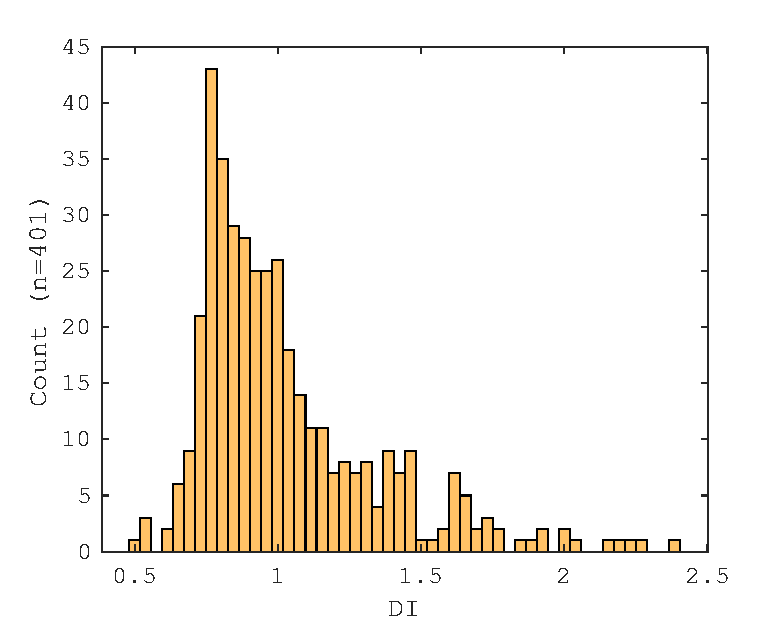
\includegraphics[max width=\textwidth]{figs/LitRev/DI.pdf}
\caption{The values of $DI$ for the 401 illuminants used by \citet{houser_review_2013}, available via \gls{PTB} as `spd\_houser', normalised such that \gls{CIE} Illuminant A receives a reference value of 1.}
\label{fig:Houser}
\end{figure}


\clearpage
\subsection{Visitor Requirements of Museum Lighting}

The visual requirements of museum visitors is likely to depend upon a large number of variables, both intrinsic and extrinsic to the visitor (e.g. intrinsic - age, cultural background, goals for the museum visit and extrinsic: luminance, lighting distribution, \gls{CCT}, \gls{CRI} and flicker properties of lighting). Some of these factors have been independently studied in a museum context, and for others it is likely that findings in other environments could generalise such that they could be used to inform decisions regarding museum lighting.

Traditionally, the principal manner in which museum professionals sought to limit damage was through setting a maximum luminance level. The implicit assumptions in this process are twofold; firstly: that damage will increase with increased luminance. This was a fairer assumption when tungsten was the only type of lighting technology, but as other lighting technologies with different \glspl{SPD} have been introduced this assumption has become less accurate (see Section \ref{sec:DamageIndex}: \nameref{sec:DamageIndex}). The second implicit assumption is that viewers will prefer higher luminance environments.

The classic study on this second assumption, performed in a mock-museum environment is that of \citet{loe_preferred_1982}. In this study Loe et al. examined three variables: painting illuminance, light source (different technologies) and light distribution. One finding from this study has had substantial impact in setting guidelines and future thinking was that a minimum of 200lux was required to `give visual satisfaction'. This figure was subsequently used in \citet{thomson_museum_1978}, which has informed a great deal of subsequent thinking on the topic. It is worth noting however, that only a small number of different luminances were sampled, and it is quite possible that the results are at the mercy of several types of bias \citep{fotios_research_2009}.

\begin{figure}[htbp]
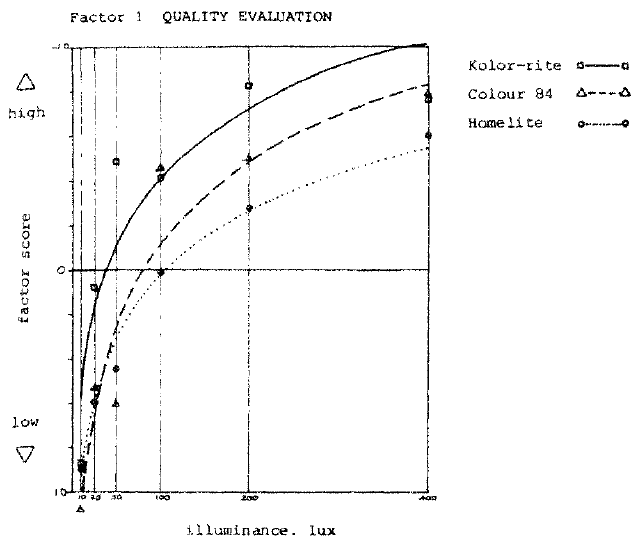
\includegraphics[max width=\textwidth]{figs/LitRev/Loe.png}
\caption{Illuminance vs a factor which is thought to indicate `quality', reproduced from \citet{loe_preferred_1982}.}
\label{fig:Loe}
\end{figure}

There has been extensive research on the visitor requirements in terms of \gls{CCT} and \gls{CRI} and these shall be covered in separate sections.

In terms of a holistic approach to museum lighting research (considering more than a single or small number of isolated variables), there has been a great deal of work which deals with the visitor experience in a broad and cultured fashion from the lofty vantage of museum studies (such as \citet{falk_museum_2016} and \citet{shapiro_museum_1990}), but rarely do the physical practicalities such as lighting get a mention. 

There notable exception, where lighting as it relates to the visitor experience is considered, is the work of Kesner in the USA in the early nineteen-nineties \citep{kesner_museum_1993-1,kesner_museum_1993,kesner_exhibition_1992,kesner_current_1991,kesner_analysis_1997}.

Kesner's studies comprised self-reporting surveys, and concluded that colour accuracy was the highest requirement and that `richness' of colour was the lowest priority\footnote{A cautious interpretation of these results is advised, considering that there were high average scores for each category.}:

\begin{quote}
\emph{``Artifact appearance, particularly clarity of artefact form and accuracy of artifact color, is the most important visitor need. Although visual impression, specifically acceptable gallery brightness and rich artefact color, is least important among the factors, it too rated highly important.''} - \citet{kesner_museum_1993-1}
\end{quote}

%more?

%Following the release of guidelines on the topic of \glspl{LED} in museums\citep{druzik_guidelines_2012}, a written survey of museum professionals who had requested these guidelines was performed, and the results reported by \citet{perrin_ssl_2014}. The respondents were predominately based in USA, with 30\% identifying as `international'. The survey was part of the USA government's `GATEWAY program'. Responding to the question `Please rank the following factors in your selection of lamps', joint first priorities are identified as `colour and spectral power distribution' and `damage potential'.

\subsection{Museum Lighting Specification Guidance Documents}

Following the interviews with the museum professionals, the five most referred-to museum lighting guidance documents were reviewed, and a summary is presented here.

\noindent
The guidelines chosen for review were:
\begin{itemize}
\item The Museum Environment \citep{thomson_museum_1986}
\item \gls{CIE} 157:2004 Control of Damage to Museum Objects by Optical Radiation \citep{cie_cie_2004}
\item Guidelines for Selecting Solid-State Lighting for Museums \citep{druzik_guidelines_2012}
\item SLL LG8: Lighting for museums and art galleries \citep{cibse_lighting_2015}
\item IES RP-30-96 Museum and Art Gallery Lighting: A Recommended Practice \citep{ies_ies_1996}\footnote{This has since been usurped by \citet{illuminating_engineering_society_ies_2017}.}.
\end{itemize}

\noindent
In summary:
\begin{itemize}
\item Recommended values were provided for:
\begin{itemize}
\item \emph{Lux}: various, dependent on sensitivity, generally based on figures from the study of visual preference by \citet{loe_preferred_1982}.
\item \emph{R$_a$}: various, most frequently \textgreater 80, with no experimental basis referenced.
\item \emph{\gls{CCT}}: various, based implicitly on \citet{kruithof_tubular_1941} or on such ideas found empirically.
\end{itemize}
\item Most also suggested visual inspection as a valid means of assessment.
\item There was often blurring between recommendations concerned with visual appearance and those concerned with conservation. 
\end{itemize}

\subsection{CCT in museums}

The \acrfull{CCT} of an illuminant describes the chromaticity of a light source on a one dimensional axis roughly from blue to yellow, based on the apparent chromaticity of a black body radiator at differing temperatures. Figure \ref{fig:BBR} shows the curve formed in chromaticity space by a set of black body radiators of different temperatures. It is worth noting that most real light sources fall upon the relatively straight section of the left-hand part of this line.

\begin{figure}[htbp]
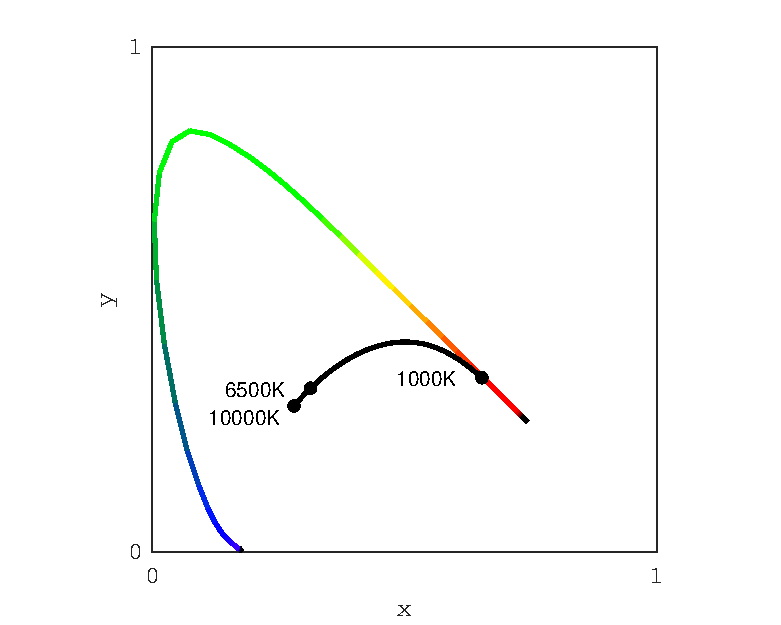
\includegraphics[max width=\textwidth]{figs/LitRev/BBR.pdf}
\caption{The black body radiator curve on a CIE 1931 chromaticity chart, highlighting \glspl{CCT} of 1000K, 6500K and 10000K.}
\label{fig:BBR}
\end{figure}

\Gls{CCT} is often described as an important variable in museum lighting, but definite recommendations, in the rare cases that they are given, are generally based on nostalgia for the appearance of tungsten lighting, questionable research on human preference \citep{kruithof_tubular_1941,fotios_revised_2017} or very rough rules that predict that damage potential will be decreased if \gls{CCT} is minimised \citep{cie_cie_2004}. Whilst some research appears to have found optimal \glspl{CCT} for viewing artwork \citep{nascimento_best_2014,pinto_correlated_2008,scuello_museum_2004,scuello_museum_2004-1, liu_cultural_2013} results often have large inter-observer variability, context dependency and it is not uncommon for the headline findings of separate studies to be in contradiction. 

Specifications often refer implicitly or explicitly to the findings of \citet{kruithof_tubular_1941}, who found that at lower levels of illumination, lower \glspl{CCT} were preferred, and that at higher levels of illumination higher \glspl{CCT} were preferred (see Figure \ref{fig:Kruithof}). Whilst this general trend seems to have anecdotal support, it is possible that there may be lighting-technology-based confounds, and recently researchers \citep{vienot_kruithofs_2009} (including a meta-study of multiple other examinations \citep{fotios_revised_2017}) found there to be no substantive support for Kruithof's findings.

\begin{figure}[htbp]
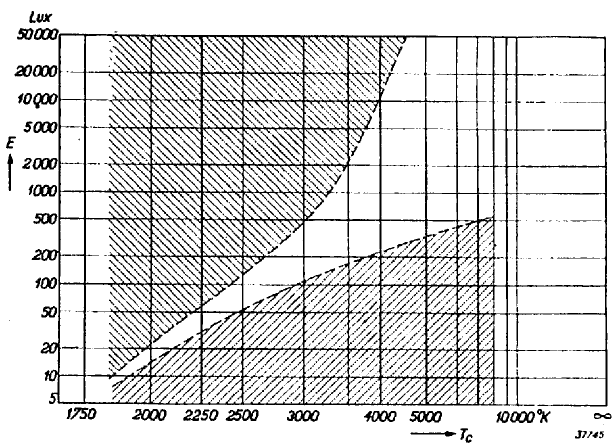
\includegraphics[max width=\textwidth]{figs/LitRev/Kruithof.png}
\caption{The `Kruithof curve' reproduced from \citet{kruithof_tubular_1941}, showing colour constancy against illuminance, and highlighting an area that is considered ``pleasing''.}
\label{fig:Kruithof}
\end{figure}

The damage justification seems more substantive; following the application of damage factors as discussed in Section \ref{sec:DamageIndex} the \gls{CIE} published a report showing the varying the \gls{CCT} of museum lighting could have a clear impact on the potential damage undergone by museum objects \citep{cie_cie_2004}. 

\begin{figure}[hbtp]
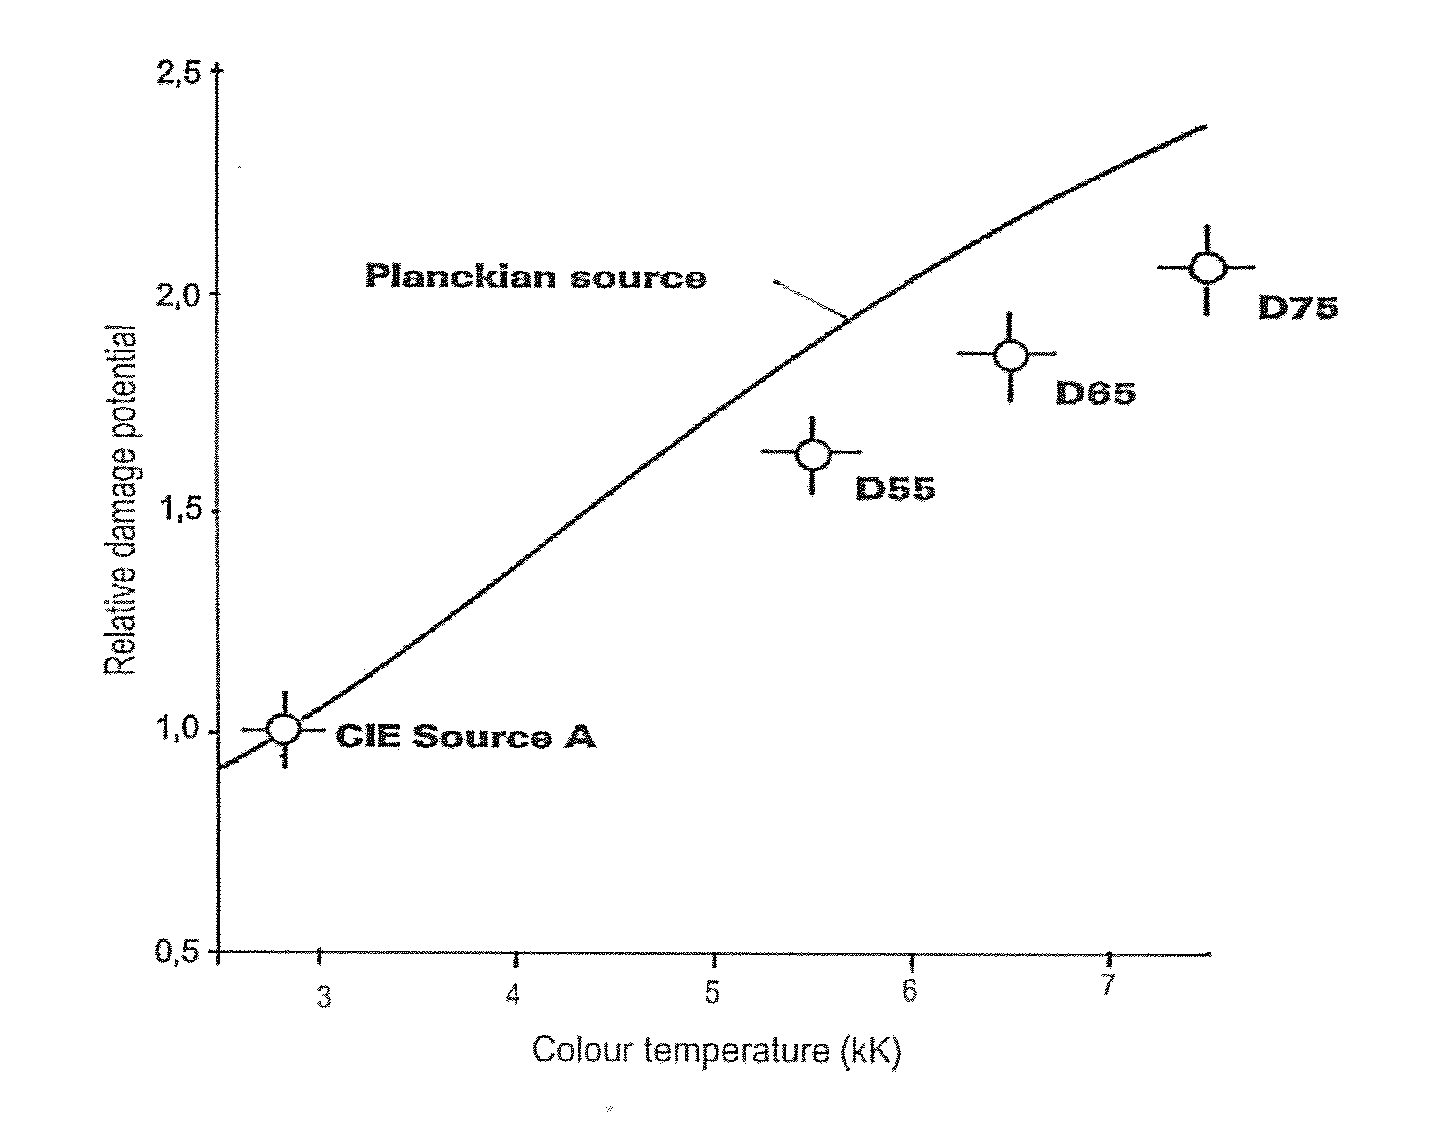
\includegraphics[max width=\textwidth]{figs/LitRev/CIE2004.png} 
\caption{Figure reproduced from CIE 157:2004 \citep[p.16]{cie_cie_2004}, showing the relationship between \gls{CCT} and relative damage potential.}
\label{fig:CIE2004}
\end{figure}

% ---------------------- %

This research relies heavily upon the applicability of damage functions to the specific materials in question. Many (my supervisors) think that damage functions are no good because they're too general, but I would be cautious about throwing the baby out with the bathwater.

\begin{enumerate}
    \item They're the best that we have.
    \item We need something with general applicability anyway - I don't see anyone providing tailored lighting for every object which exists.
    \item The physics checks out.
    \item They're definitely applicable to at least some objects.
\end{enumerate}

To verify the findings of the \gls{CIE}, to extend their findings to \glspl{LED}, and to provide code for others to do similar research or even test their own lights/materials, I wrote some code\footnote{\url{https://github.com/da5nsy/DamageIndex/blob/c7851e27ca1b0915013d8723db04704b49b4085e/CalcDI.m}} which would calculate a \gls{DI}. Then I used that code to compute a new version of the \gls{CIE} plot.

%\afterpage{\clearpage}
%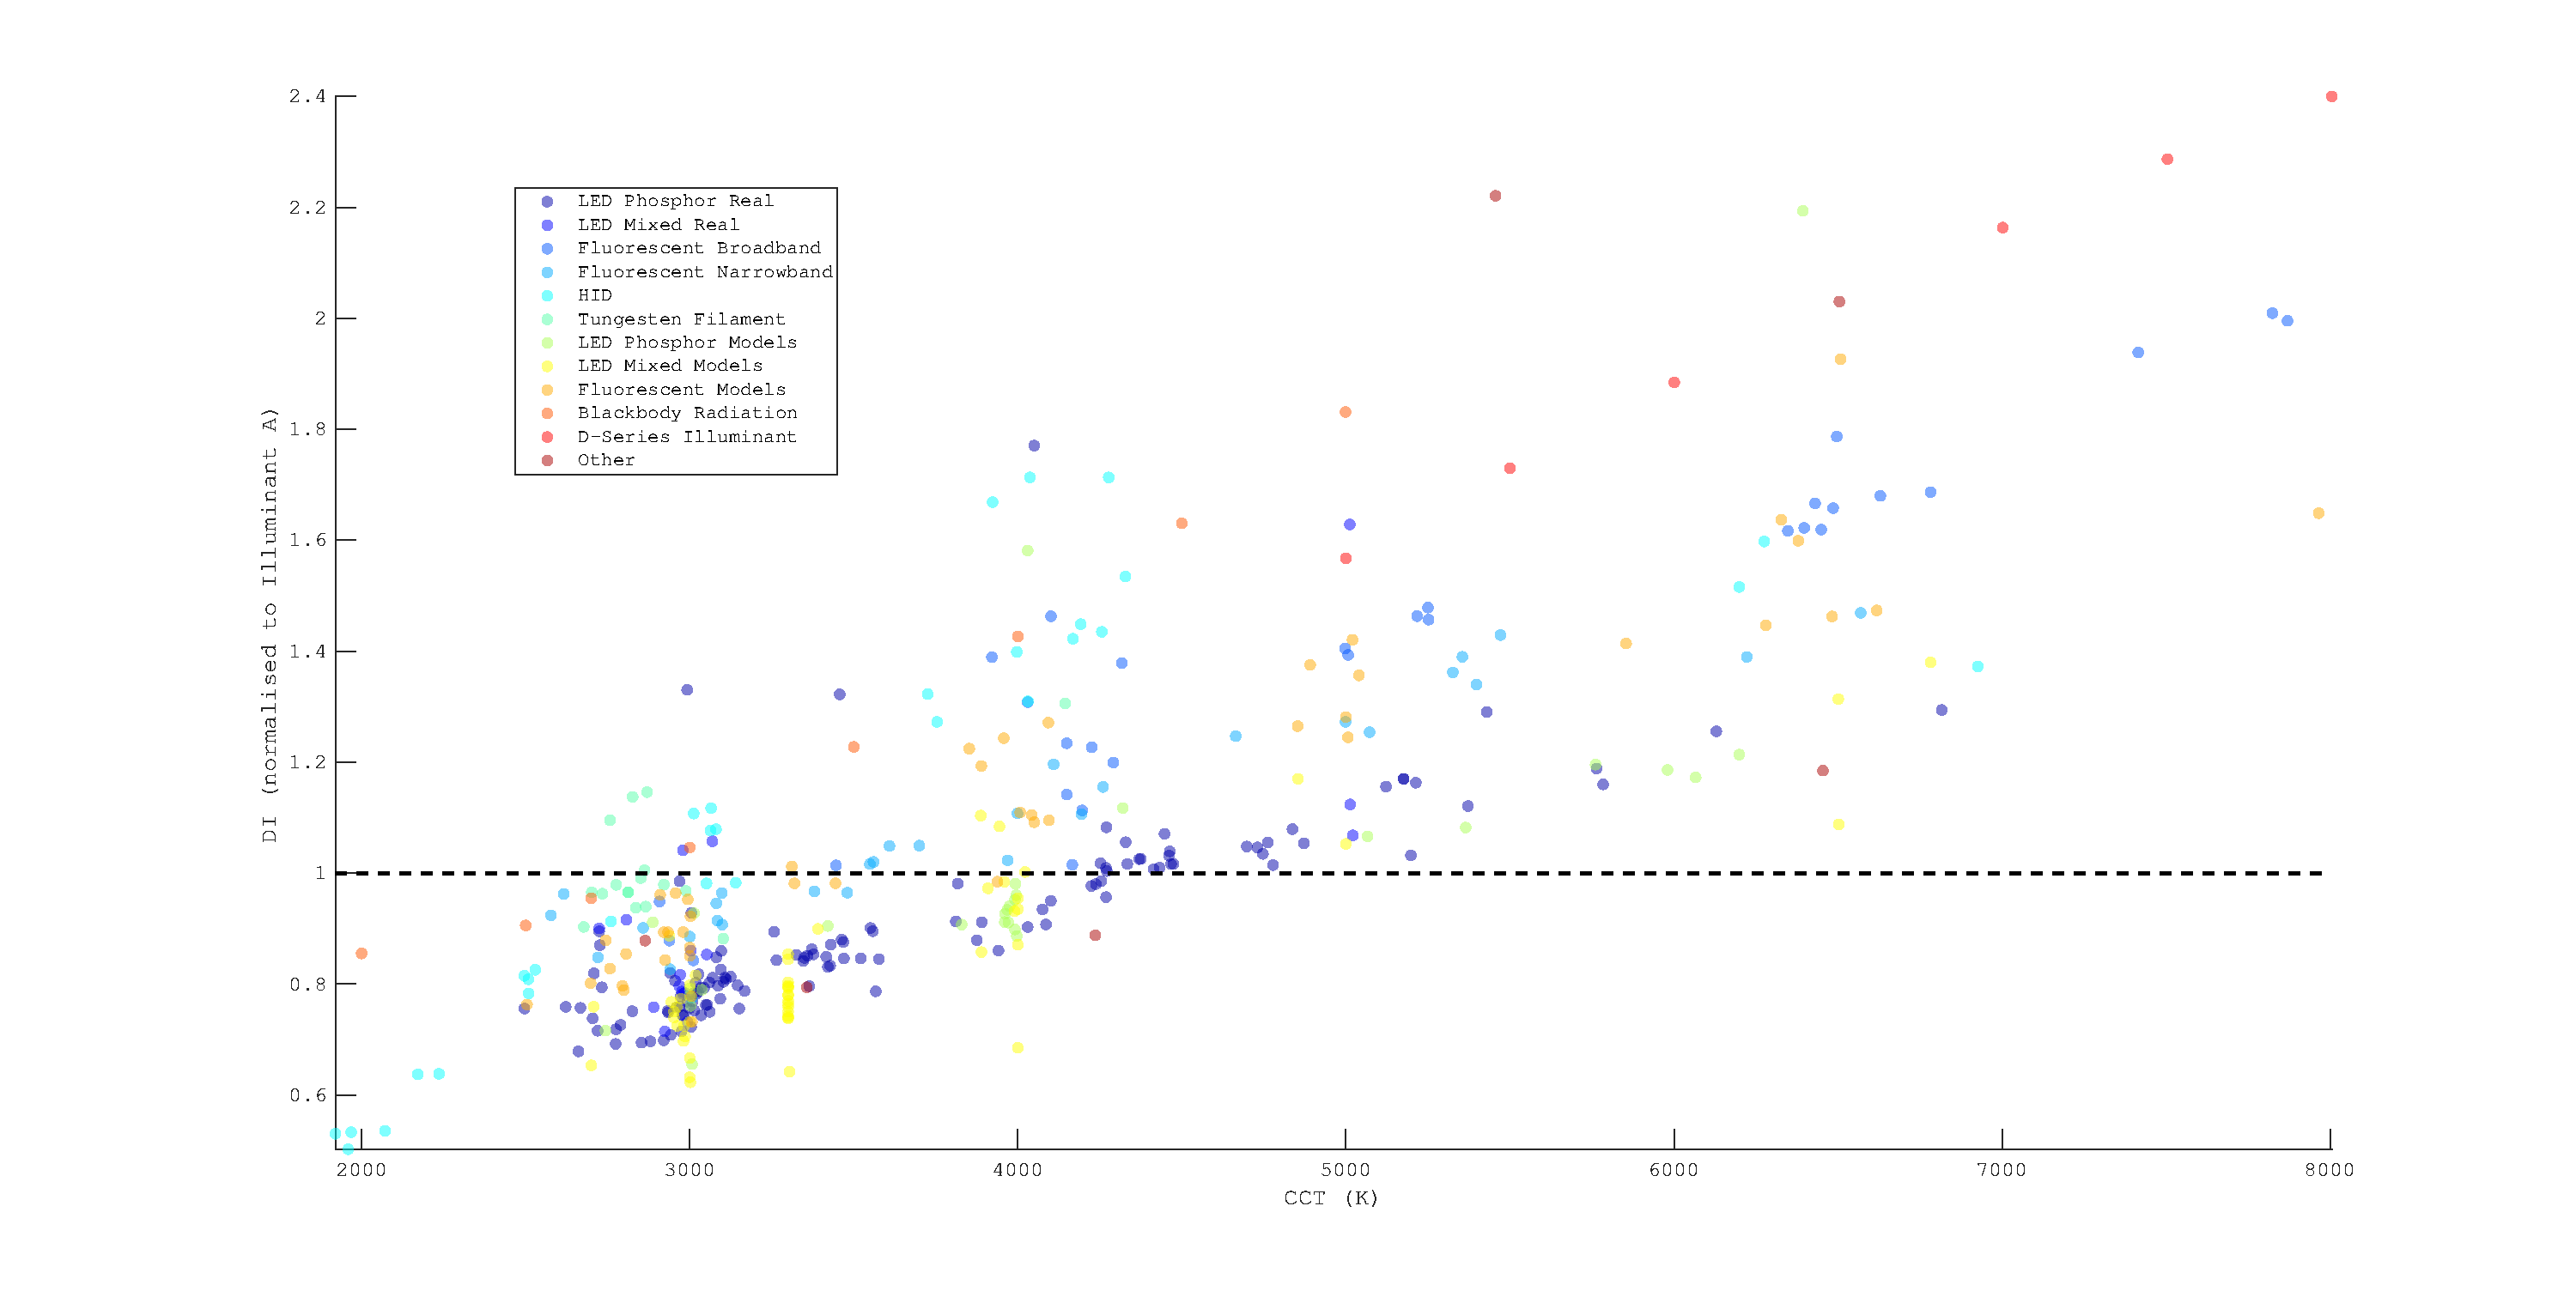
\includepdf[pages=-,rotate=90, offset=75 -75]{figs/LitRev/CCTvsDI.pdf}
% \begin{figure}[t]
%     \caption{The \glspl{CCT} and \glspl{DI} of the \glspl{SPD} used by \citet{houser_review_2013} [provided via personal communication, but now partially available via \gls{PTB} as `spd\_houser'].}
%     \label{fig:CCTvsDI}
% \end{figure} 

\begin{fullpagefigure}
\figpdf[pages=-,rotate=90, offset=75 -75]{figs/LitRev/CCTvsDI.pdf}
%\figpageside{}
\caption{The \glspl{CCT} and \glspl{DI} of the \glspl{SPD} used by \citet{houser_review_2013} [provided via personal communication, but now partially available via \gls{PTB} as `spd\_houser'].}
\label{fig:CCTvsDI}
\end{fullpagefigure}

The results of these computations show a clear relationship between \gls{CCT} and \gls{DI}. Considering that this is not currently taken advantage of in museum lighting, it seems as though there is a great potential for reducing damage whilst maintaining visitor visual satisfaction.

%\clearpage
% This is combo with the figpageside thing above currently isn't quite working

\subsection{Colour Rendering Indices in Museums}

Are fidelity indices suitable for museum use? 
The first chapter of Cuttle's book `Light for Art's Sake: Lighting for Artworks and Museum Displays'19 is titled `A philosophy for the presentation of art'. The choice of title here is apt but may surprise some readers, sounding more whimsical than might be expected of a serious subject attended by scientists and engineers. The reason it is so apt is because lighting is unavoidably a creative intervention (I owe this phrase to Katherine Curran); which is to say that there is no lighting which is truly impartial, and no lighting which is truly correct in the sense of being unequivocally superior to another. All lighting decisions require choices to be made, and whilst these choices can be wrapped up to appear as an optimization problem where proximity to a particular solution is the goal, the problem always rests on the bedrock of a philosophy based decision.

In the above mentioned chapter Cuttle lays out a total of seven distinct philosophical propositions, which he poses for consideration as approaches to museum lighting, some contradictory and some with the potential to overlap:

1.	`To make the artwork appear as it would have appeared to the artist at the time of its creation
2.	To ensure that no damage due to light exposure will occur
3.	To achieve the best possible appearance of the artwork
4.	To provide optimum conditions for viewing art
5.	To impart a sense of having seen `the real thing'
6.	To assist viewers to understand the displayed objects and their reason for being there
7.	For the lighting designer to establish a distinct and recognisable style'19 

These propositions refer to museum lighting holistically, considering all aspects of museum lighting, but can be readily focused on the problem of colour appearance specifically. Before we narrow our gaze however, it is worth briefly considering a wide view of lighting attributes which may aid in the realisation of `good quality' museum lighting. Consider Scott Rosenfeld's list of the five `controllable qualities' in museum lighting; `intensity, movement [temporal artefacts], angle [modelling, avoiding glare and reflections], distribution [ambient lighting vs. spot lighting], color'20.
Whilst Cuttle's propositions make for interesting discussions and enjoyable extended pondering, they are of limited assistance in the practical task of actually specifying lighting. Thankfully, a range of tools exist for the examination of the colour rendering properties of a light source, in the form of indices which aim to numerically describe an illumination's effect on colour appearance of the objects of which it is tasked with illuminating.

Traditionally, colour rendering indices aim to offer a standardized method for calculating the colour differences induced by the substitution of a reference illuminant with a specific test source, and for comparing the relative merit of different test light sources on their ability to induce minimum change. In modern parlance this type of index should be referred to as a colour fidelity index, that is- one which is conceptually concerned with colorimetric reproduction. The term `colour rendering' has come to encompass much more than just fidelity.

Diametrically opposed in some ways to fidelity are the indices which aim to quantify `preference'. In the simplest case, a preference index will aim to provide a value that is predictive of how an observer would rate a light source it against other light sources. 

Within, and on the spectrum between these two groups there exist a range of different indices with subtly different aims and mechanisms for achieving these aims. For a thorough overview, albeit one which omits some more recent developments, see Guo and Houser21.

In practice, both of these philosophical approaches are mandated in current lighting guidance. For the most part, advice for lighting specification6,7 on the subject of colour rendering can be simplified to read `use lamps of above \gls{CRI} 80 (referring tacitly to \gls{CIE} R$_a$) but always test them visually before you buy in bulk'. Whilst this may at first seem like sensible advice, upon further inspection it in fact represents a serious contradiction, unless considered with heavy caveats. The problem rests in the fact that \gls{CIE} R$_a$ is a fidelity index, whereas any visual inspection is likely to be performed by observing the appearance of an object under the test illumination without a reference. Fidelity aims to describe accuracy of reproduction, but this is a quality which is arguably not testable by visual inspection. This contradiction seems to perpetuate unnoticed in museum practice, with lighting specifiers often abstractly declaring to target a faithful/accurate/honest/impartial representation of objects, but practically choosing light sources based on visual inspection where preference is the only criteria. There is of course a range of approaches, ranging from pure reliance on indices to almost entire reliance on visual testing.

In conclusion, no one metric exists that would satisfy the divergent aims and philosophies of museum lighting. Several distinct types of colour rendering index exist, but the existing range fall into the broad categories of `fidelity' or `preference', with the latter being particularly poorly definable due to its variability in different environments, with different user functional requirements and different intrinsic preferences between different observers. Progress could be made by breaking these broad categories into smaller more manageable specific objectives.

\clearpage


%%%% BONUS AREA %%%%%%%%%%


%\subsection{LEDs in museums}

%%%%%%%%%%%%%%%

%Theoretically, there exists a division between recommendations which deal with visual appearance and those which deal with physical degradation; the first group supported by the science of human vision, and the second supported by material sciences and chemistry. Whilst it is important to be aware of this distinction, it is normally not possible to consider them entirely separately in practice, as many variables will affect both.

%%%%%%%%%%%


%Extending the question of visibility is the subject of appearance. It is a general expectation that museums represent objects in a truthful and impartial manner, and it seems sensible that decisions concerning the appearance of items in museums should be made with this in mind. Alongside this, many museums treasure items where part of their value is aesthetic2, and it follows therefore that a technique which aids in the beautification of an object might be of interest, and this might be particularly of interest if the object is known to have deteriorated since the time of production.

%%%%%%%%%%%

% \subsection{Lighting at The British Museum}

% Lighting at the British Museum has developed in a somewhat organic manner, from the early days of the museum before the introduction of artificial lighting. This leaves the museum with more than sufficient daylight in most spaces during daylight hours, where the increased modern knowledge regarding the deleterious effect of lighting now means that conservators must find ways in which to limit this natural resource so that objects are not unduly exposed. 

% The gallery lighting is replaced when a gallery is refurbished, and the latest technology is installed when a new gallery is created, where viable in terms of suitability and considering financial limitations. Other than this, lighting technologies tend to not be updated other than to replace individual lamps. This coupled with the grand scope of the museum, which means that it is rare for multiple galleries to be refurbished simultaneously, has led to a vast array of lighting designs and technologies. It in fact appears to represent a rather special example of `museum lighting through the ages', with daylight, tungsten, fluorescent and metal halide lamps all seemingly represented, as well as various illumination geometries reminiscent of the times of their fitting. It should be noted that these assertions are made following empirical observation with spectrophotometers and not from conversations with museum staff, see section 3.3 Collection of \gls{SPD} Data at British Museum.

% There also seems to be a great range of lighting quality within the British Museum, with some spaces feeling bright and others comparatively gloomy. There is a range of colour temperatures and chromaticities of light at the museum, as shown in Figure 1.

% Multiple methods are currently employed to limit the exposure of objects in the museum. \Gls{UV} absorbing film or glazing which incorporates \gls{UV} reduction is used throughout the museum and in certain galleries there are automatic blinds which limit the intrusion of direct sunlight at specific times of the day and year. For particularly sensitive objects, rooms are lit artificially at very low levels, and some objects are selectively lit in order to further limit their accumulative exposure.

% 